\documentclass[12pt, a4paper]{article}

\usepackage[pdftex]{graphicx}

\usepackage{graphs-tikz}

%------------------------------------------------------------------------------------------------------------------------------------
%------------------------------------------------------------------------------------------------------------------------------------
\begin{document}

Graphs for tikz. Examples.

\bigskip

\begin{center}
\begin{tikzpicture}
	\thickSpider[fill=black]{0}{0}{1}{5}{f};

	\thinSpider{5}{0}{1}{8}{f};
\end{tikzpicture}
\end{center}

\bigskip

\begin{center}
\begin{tikzpicture}
	\cycle[size=medium, color=red, fill=red!20]{0}{0}{1.25}{6}{c};

	\complete{5}{0}{1.25}{6}{k};
\end{tikzpicture}
\end{center}

\bigskip

\begin{center}
\begin{tikzpicture}
	\vertex[green]{0}{0}{v};

	\vertexLabel[above]{v}{N};
	\vertexLabel[green, above right]{v}{NE};
	\vertexLabel[right]{v}{E};
	\vertexLabel[green, below right]{v}{SE};
	\vertexLabel[below]{v}{S};
	\vertexLabel[green, below left]{v}{SO};
	\vertexLabel[left]{v}{O};
	\vertexLabel[green, above left]{v}{NO};
\end{tikzpicture}
\hspace{50pt}
\begin{tikzpicture}
	\complete[color=blue]{0}{0}{1.5}{7}{K};

	\vertexLabel[below, inner sep=7pt]{K1}{$v_1$};
	\vertexLabel[below, inner sep=7pt]{K2}{$v_2$};
	\vertexLabel[below left]{K3}{$v_3$};
	\vertexLabel[above left]{K4}{$v_4$};
	\vertexLabel[above, inner sep=5pt]{K5}{$v_5$};
	\vertexLabel[above right]{K6}{$v_6$};
	\vertexLabel[below right]{K7}{$v_7$};

	\edgeLabel[red, below left, inner sep=1pt]{K2}{K3}{$e$};
\end{tikzpicture}
\end{center}

\bigskip

\begin{center}
\begin{tikzpicture}
	\vertex[size=big]{0}{0.75}{v1};
	\vertexLabel{v1}{$v_1$};
	\vertex[size=big]{0}{1.75}{v2};
	\vertexLabel{v2}{$v_2$};
	\vertex[size=big]{1}{2.75}{v3};
	\vertexLabel{v3}{$v_3$};
	\vertex[size=big, fill=blue!20]{2}{1.75}{v4};
	\vertexLabel{v4}{$v_4$};
	\vertex[size=big]{2}{0.75}{v5};
	\vertexLabel{v5}{$v_5$};

	\edge[color=red, line width=4pt]{v1}{v2};
	\edge[line width=3pt]{v2}{v3};
	\edge[dashed]{v3}{v4};
	\edgeCurved{v4}{v5}{0}{0};
	\edgeCurved[dashed, color=blue, line width=2pt]{v5}{v1}{180}{270};
	\edgeLabel[below, inner sep=18pt]{v5}{v1}{$e_{1,5}$};
\end{tikzpicture}
\hspace{50pt}
\begin{tikzpicture}
	\vertex{0}{0.5}{a1};
	\vertex{0}{1.5}{a2};
	\vertex{0}{2.5}{a3};
	\vertex[blue]{1.5}{0}{b1};
	\vertex[blue]{1.5}{1}{b2};
	\vertex[blue]{1.5}{2}{b3};
	\vertex[blue]{1.5}{3}{b4};

	\join[red, dashed]{a}{3}{b}{4};
\end{tikzpicture}
\hspace{50pt}
\begin{tikzpicture}
	\vertex[size=medium]{0}{0}{g00};
	\vertex[size=medium, fill=black!20]{0}{1}{g01};
	\vertex[size=medium, fill=gray]{0}{2}{g02};
	\vertex[size=medium, pattern=north east lines, pattern color=black]{1}{0}{g10};
	\vertex[size=medium, pattern=north west lines, pattern color=black]{1}{1}{g11};
	\vertex[size=medium, pattern=dots, pattern color=black]{1}{2}{g12};
	\vertex[size=medium, pattern=horizontal lines, pattern color=black]{2}{0}{g20};
	\vertex[size=medium, pattern=vertical lines, pattern color=black]{2}{1}{g21};
	\vertex[size=medium, pattern=grid, pattern color=black]{2}{2}{g22};

	\edge{g00}{g01};
	\edge{g00}{g10};
	\edge{g01}{g02};
	\edge{g01}{g11};
	\edge{g02}{g12};
	\edge{g10}{g11};
	\edge{g10}{g20};
	\edge{g11}{g12};
	\edge{g11}{g21};
	\edge{g12}{g22};
	\edge{g20}{g21};
	\edge{g21}{g22};
\end{tikzpicture}
\end{center}
%-------------------
\end{document}
